\section{Computational Methods and Software}
\label{sec:software}

% \begin{itemize}
%  \item \st{discretized equations, finite elements, stabilized}
%  \item penalty formulation, also consider discussing sep model
%  \item \st{software (GRINS+Libmesh)}
%  \item \st{verification of software}
%  \item \st{tool-chain, simulation machine and hardware}
%  \item \st{simulation geometry and boundary conditions for wind/thermal-only}
% \end{itemize}

\subsection{Discretization Scheme}

To solve the Navier-Stokes equations on a computer, a
Galerkin finite element method (FEM) is used, with linear basis
functions for both the velocity and pressure. This scheme circumvents
the Babuska-Brezzi conditions\cite{bb-cond} and 
uses equal-order elements for velocity and 
pressure,  by introducing a stabilization term as first described by
Hughes\cite{Hughes198685} and extended to natural convection as in
Becker and Braack\cite{Becker2002428}.  

The system of ODEs are discretized in time using a theta-method. 
Newton iterations are used to for solve the resulting nonlinear problem. 
The unsteady solver used is typically backward Euler for the
corresponding stability regardless of timestep size. 

\subsection{Penalty Method Implementation}

In the previous section it was noted that a penalty method is used to
represent impermiable surfaces such as the wind block cone. Babuska's
penalty treatment of constraints\cite{1973fempen,ZAMM:ZAMM19880680925}
is used. This was selected because it is easily imposed in the FEM
context, and the method has been explored in detail in the literature. 

In this approach, a penalty for violating the constraint is included in
a variation formulation. As an example, consider Laplace's equation on a
domain $\Omega$ with boundary $\partial\Omega$, 
\begin{equation}
 \nabla^2 u = 0. 
\end{equation}
Dirichlet boundary conditions are introduced into the weak form
\begin{equation}
 u|_{\partial \Omega} = g
\end{equation}
which becomes 
\begin{equation}
\int_{\Omega}  - \nabla u \cdot \nabla v dx - \frac{1}{\epsilon}
 \int_{\partial \Omega} (u-g) \cdot v ds = 0 \quad \forall v \in H^1
\end{equation}
where $\frac{1}{\epsilon}$ is the penalty parameter. This is the weak
form for Laplace's equation with a Robin boundary condition 
\begin{align}
 u = g - \epsilon \partial_n u. 
\end{align}
For sufficiently small $\epsilon$, the original Dirichlet boundary
conditions will be satisfied approximately. Clearly, $\epsilon$ has
units of length, and can be interpreted as a ``slip length''. In the
Navier-Stokes solver, this penalty formulation is used to approximately
impose the no-flow through for impermiable surfaces, such as the
cone.\todo{need explicit mathematical description of exactly the formulation}

\subsection{Simulation Geometry and Boundary Conditions}
\label{sec:bc}

%
% be sure to mention the 'sponge' layer. would also be nice to have
% references to papers on it! 
%

All simulations are performed in a cuboid domain, with 6 faces. We
use a uniform mesh in the lateral directions, and a non-uniform mesh
in height to resolve the boundary layer. The meshes are scaled by system
diameter. The same number of grid points are used for every
simulation, with the total domain extents scaled up with system size. In
this way the ratio of the domain diameter to system diameter remains
fixed. Likewise, the diffusivities are proportionally scaled with grid
size to ensure that the cell Reynolds number is maintained for
every simulation. After operation, solutions are evaluated to ensure
that the qualitative character of the solution does not
change.\todo{define cell reynolds number here}


%
% explain how cell reynolds number is maintained for each grid
%

For the ``thermal-only'' case study (no mean wind), 
periodic boundary conditions are used on the four sides, a modified
neumann condition on the top boundary, and dirichlet boundary conditions
on the bottom (the ground).\todo{write down the math} 
These are shown schematically in Figure
\ref{fig:thermalbc}. On the ground, a ``no-slip'' velocity boundary
condition is imposed on the velocity field, and a dirichlet condition
uniformly fixes the temperature of the surface. 

The modified neumann condition is necessary due to the presence of both
inflow and outflow across the face. In the region approximately above
the vanes, the concentrated hot plume is lifted by buoyancy
upward and out of the simulation domain. However, the radial inflow
towards the apparatus is drawn in by large scale convection cells larger
than the system diameter. Thus, our boundary conditions must permit
inflow along the areas above and external to the vanes. To avoid an
ill-posed problem, the ``v'' and ``u'' components of inflow velocity are
set to zero.  

Finally, a ``sponge layer'' is labeled near the top boundary. 
This layer
artificially increases the momentum diffusivity by up to ten times the nominal
value. This was designed in response to instabilities in the modified
neumann boundary condition that occurred when small, high velocity fluid
parsels would exit the top. This would create high velocity inflows, and
the feedback loop would result in numerical blow-up. Mindful of the fact
that the character of solution not important in this region, and that
our physical interest remains focused on the region inside and
in immediate proximity to the vanes, we introduced a higher diffusivity
``sponge'' region that would diffuse the high velocity exiting jets
sufficiently to prevent numerically un-physical behavior. No results are
quoted from this ``sacrificial'' region, as it is not considered
meaningful. These regions are referred to by many names in the
literature\cite{doi:10.1146/annurev.fluid.36.050802.121930}, such as
absorbing layers, fringe regions, buffer zones, sponges, etc.

\begin{figure}[!htb]
  \begin{center}
    \includegraphics[width = 8 cm]{figs/thermal_only}
    \caption{Boundary conditions for the thermal-only scenario. }
    \label{fig:thermalbc}
  \end{center}
\end{figure}

The wind cases are diagrammed in figures \ref{fig:windstream} and
\ref{fig:windspan}. The wind case has a proscribed inlet boundary layer
for both the temperature profile as well as the velocity. The velocity
boundary layer is set to the common 7th power function for a
turbulent boundary layer,  
\begin{equation*}
  u_{in}(z) = U \text{ min }\left(\left(\frac{z}{\delta}\right)^7,1\right)
\end{equation*}
where $\delta$, the boundary layer thickness, is set based on data
measured by our experimental partners in the field. 
The thermal boundary layer is assumed to have a similar boundary layer,
but, as observed in real atmospheric flows, there remains a vertical
temperature gradient outside the thin boundary layer. Based on
literature a $2/3$ Kelvin per meter gradient has been
selected\cite{Blocken2007238}. The sides, outflow and top are all set to
modified neumann boundary conditions, as described above. The outflow
region in the back also needs the modified neumann as it does
occasionally exhibit mild inflow on account of the unsteady wake. Sponge
layers are set along the top and back (outflow) of the box. 

%
%335+18*tanh(-z/0.1)-z*2/3
%
\begin{figure}[!htb]
  \begin{center}
    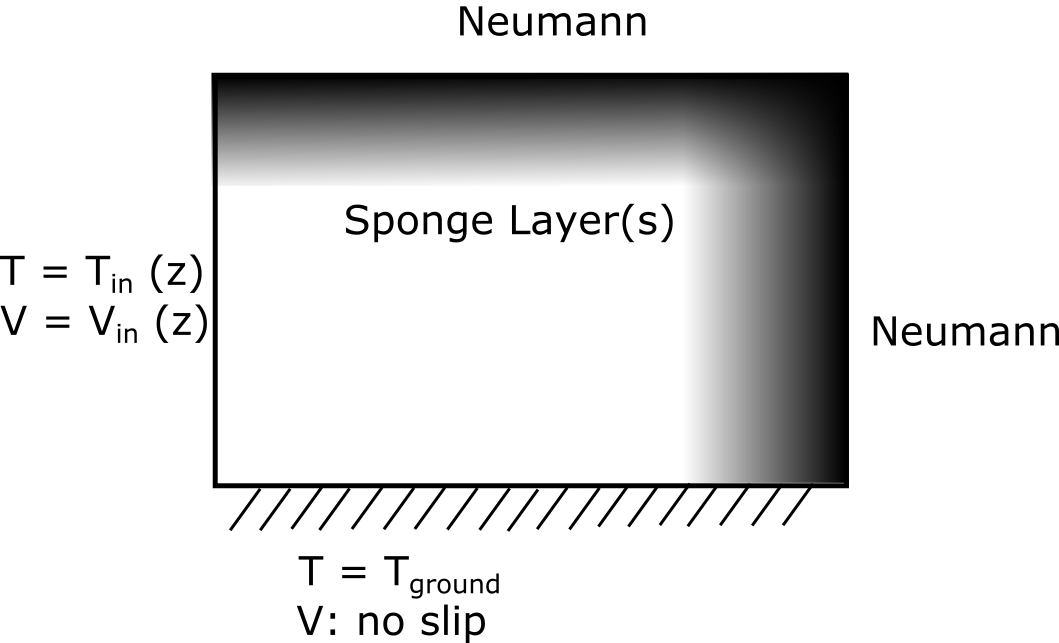
\includegraphics[width = 8 cm]{figs/wind_streamwise}
    \caption{Boundary conditions for the wind and thermal scenario, in
   the streamwise direction.} 
    \label{fig:windstream}
  \end{center}
\end{figure}

\begin{figure}[!htb]
  \begin{center}
    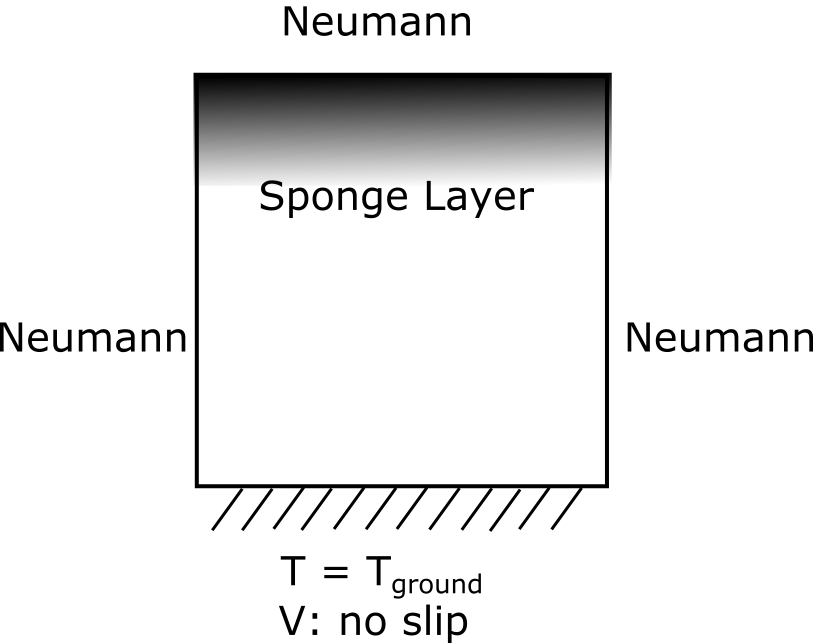
\includegraphics[width = 8 cm]{figs/wind_spanwise}
    \caption{Boundary conditions for the wind and thermal scenario, in
   the spanwise direction. } 
    \label{fig:windspan}
  \end{center}
\end{figure}


\subsection{Software Stack}

The numerical approximations described above were implemented using the
GRINS library\cite{GRINSpaper} in Libmesh\cite{libMeshPaper}. 
It was designed to support multiphysics FEM
applications, the reusability and extensibility of mathematical
modeling kernels, supporting interfaces to existing solver and
discretization libraries to enable modern solution strategies, while, at
the same time, retaining flexibility to effectively address a wide range
of science or engineering problems. 

GRINS provides a platform that enables powerful numerical algorithms
such as adjoint-based AMR, adaptive modeling, sensitivity analysis,
and, eventually, enabling uncertainty quantification. While few of these
capabilities are in use for the present work, they could be useful in
future investigations. 

GRINS stands for, ``General Reacting Incompressible Navier-Stokes'',
which roughly encapsulates the physical regimes it was originally
designed to simulate. GRINS is open-source, and available on
\hyperref[www.github.com/grinsfem/grins]{github}. It is released 
under LGPL2.1.  GRINS is heavily unit tested, with over 60 tests
available to ensure the reliability of results regardless of install platform.

%The remainder of this subsection is devoted to
%discussing the underlying libraries used and the description of the
%GRINS framework.  
% PETSC\cite{petsc} trilinos\cite{trilinos}

% GRINS also uses the fparser\cite{fparser}
% library to support both parsing and compilation of mathematical
% functions into high 
% performance kernels. This capability allows for easy specification of
% boundary conditions, initial conditions, or constitutive equations from an input file. 

% Currently, libMesh has been scaled tens of thousands of cores and has
% been run on over 100,000 cores on the BG/Q machine Mira at Argonne National
% Lab\cite{libmesh-scaling}

%In principle, alternative software libraries/frameworks such as
%FEniCS\cite{fenics}, OpenFOAM\cite{openfoam}, etc. would likely be
%capable of simulating this regime. 


\subsection{Tool Chain and Simulation Custodianship}

Runs are queued on Texas Advanced Computing Center (TACC)
supercomputer's Lonestar Four and Stampede. Run durations are typically  
twelve hours to perform several hundred timesteps. 
These runs are generally submitted to the production queue and are  
264-528 processing cores, 
or 22-44 nodes on Lonestar (with 12 cores per node), and a similar number
for Stampede. The runs typically have several million degrees of freedom (DoF), 
and the local number of DoF per core is maintained at $O(10^4)$. This was
selected due to memory considerations, after a strong scaling
analysis of the performance of the code on these resources, and
after consulting with the software developers.  

After a run terminates, several scripts are automatically invoked. 
These scripts archive the run (outside of the volatile /scratch 
production directories) and simultaneously, label the concluded run with
unique metadata that defines the system environment, the jobs input
files and run definitions, as well as information detailing the
hypothesis or physics the job was intended to investigate. Finally, once
a week a script performs \textbf{rsync} on the entire archived database to
ensure more than single redundancy for the runs. 

In other words, the workflow is sufficiently advanced as to permit
rapidly queuing a series of runs (in parallel) to
investigate a variety of conditions or scenario parameters. This
capability is necessary for the optimization campaign detailed in
\ref{sec:proposed_work}, where running many concurrent investigations
will be required to adequately sample the configuration space. 
